\documentclass[border=5pt, multi, tikz]{standalone}
\usetikzlibrary{quotes,arrows.meta}
\begin{document}
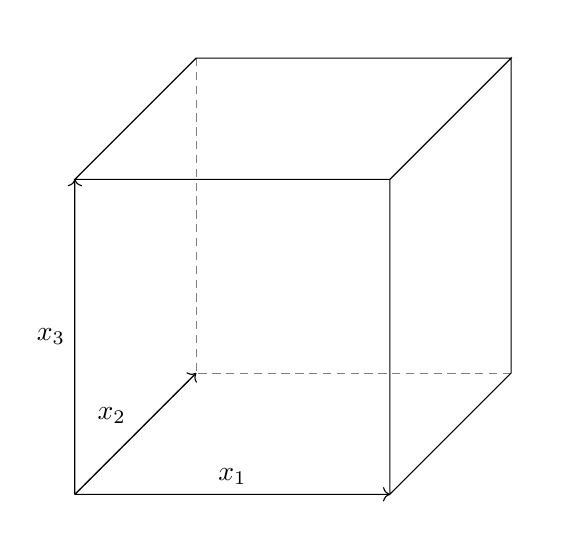
\begin{tikzpicture}[every edge quotes/.append style={auto, text=black}]
\pgfmathsetmacro{\cubex}{4}
\pgfmathsetmacro{\cubey}{4}
\pgfmathsetmacro{\cubez}{4}
\draw [draw=black, every edge/.append style={draw=black, densely dashed, opacity=.5}, fill=white]
(0,0,0) coordinate (o) -- ++(-\cubex,0,0) coordinate (a) -- ++(0,-\cubey,0) coordinate (b) edge coordinate [pos=1] (g) ++(0,0,-\cubez)  -- ++(\cubex,0,0) coordinate (c) -- cycle
(o) -- ++(0,0,-\cubez) coordinate (d) -- ++(0,-\cubey,0) coordinate (e) edge (g) -- (c) -- cycle
(o) -- (a) -- ++(0,0,-\cubez) coordinate (f) edge (g) -- (d) -- cycle;
\path [every edge/.append style={draw=black, |-|}]
(b) edge [->, "$x_1$"] (b -| c)
(g) edge [<-, "$x_2$"'] (a |- c)
(b) edge [->, "$x_3$"] (b |- a)
;
% just for alignment
\node at (-4.6, -4.5, -.8) {$\phantom{\underline{0}}$};
\node at (2.3, 2.2, 1.4) {$\phantom{\underline{1}}$};
\end{tikzpicture}
\end{document}